\chapter{Analyse d'une des publicités}

\label{Analyse d'une des publicités}

\section{Présentation de la publicité analysée}

De ce contexte, né en 1964, de la plume de l'illustrateur New-Yorkais \textit{Haddon Sundblom}, la réclame qui nous intéresse.

\begin{figure}[th]
\centering
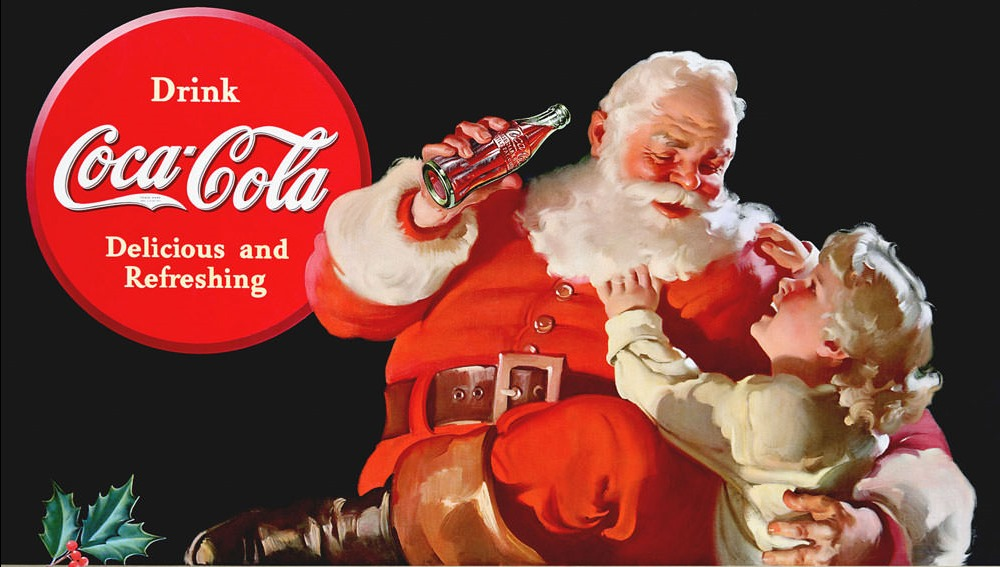
\includegraphics[width=130mm]{medias/affiche_coca}
\decoRule
\caption{Réclame étudiée dans cette partie.}
\end{figure}

J'ai choisi cette publicité en particulier car elle résume en idées simples tout les messages que l'entreprise souhaitait faire passer pendant cette période de son histoire.

%----------------------------------------------------------------------------------------

\section{Analyse descriptive de la publicité}

\subsection{Une présentation sobre}
On voit tout d'abord qu'il n'y a aucun élément superflu, le fond est noir, ce qui nous fait comprendre que cette réclame veut uniquement montrer ce qu'elle a à dire, mettant d'avantage en avant ses propos. Tout élément ici a donc son importance; À première vue, on remarque entre-autres, trois éléments principaux dans la composition: le père noël, ayant une place centrale quoique légèrement déportée par la droite afin de laisser place au logo coca-cola, dans un cercle rouge avec deux slogans. On pourrait aller jusqu'à formaliser et penser que l'utilisation du cercle rouge n'est pas dû à un simple hasard mais bien au rappel des capsules de bouteilles en verre, renforçant d'avantage de façon non-consciente la marque dans nos esprits.
\subsection{Une présentation attrayante}
Le fond noir ne sert pas qu'à mettre en avant les éléments, mais fait même mieux ressortir les couleurs prédominantes de la marque. On remarque que tout est aussi fait pour associer le bonheur avec la boisson, en particulier avec le sourire des personnages.
\subsection{Un rappel des thèmes hivernaux}

%----------------------------------------------------------------------------------------

\section{Le but de la publicité}

\subsection{"\textit{Drink Coke}"}
Il faut avant tout savoir quel est le but de cette opération; En effet, on peut grossièrement catégoriser les types de publicités en trois catégories, toutes aux ambitions bien différentes :
\renewcommand{\labelitemi}{$\bullet$}
\begin{itemize}
\item La publicité argumentation : elle défend une idée et/ou tente de modifier l’opinion des récepteurs.
\item La publicité informative : elle a pour fonction de livrer au récepteur une information.
\item La publicité incitative : ce type de publicités poussent les gens à agir et à acheter un produit
\end{itemize}
On remarque que la stratégie commerciale qu'emploie Coca-Cola tient de l'ordre de la publicité incitative:
on le remarque tout d'abord dans ce qui était leur slogan que l'on retrouve sur cette publicité, "\textit{Drink Coca-Cola.}" ("\textit{Bois Coca-Cola.}"), qui ressemble fortement à une sorte d'ordre voire d'injonction que le consommateur reçoit. De plus, on remarque que cette méthode agressive transparaît aussi dans d'autres slogans, comme par exemple en 1952 avec "\textit{What you want is a Coke.}" ("\textit{Ce que vous avez besoin, c'est d'un Coca-Cola.}").
On cherche donc à aguicher le consommateur par 